\documentclass[a4paper,12pt]{article}

\usepackage{graphicx}   % For including images
\usepackage{setspace}   % For line spacing
\usepackage{geometry}   % To adjust margins
\usepackage{ragged2e}
\usepackage{array}
\usepackage{caption}
\geometry{margin=1in}   % Set margin size

\begin{document}

\begin{center}
    \textbf{\huge{CS702 - COMPUTING LAB}} \vspace{2cm}

    \Large{A REPORT ON THE PROJECT ENTITLED} \vspace{1cm}

    \textbf{\LARGE{COVERSATIONAL USED CAR PRICE PREDICTOR}} \vspace{2cm}
\end{center}

\begin{center}
    
\includegraphics[width=0.3\textwidth]{logo.jpeg} % Specify the path to your logo image
\end{center}

\vfill

\noindent
\begin{center}
    \textbf{Group Members:} \\
    \vspace{0.5cm}  % Adds a bit of vertical space
    \begin{tabular}{c @{\hspace{3cm}} c}  % Creates two columns with 3cm space between them
        \textbf{ABHIJITH C} & \textbf{ANAND M K} \\
        \textbf{242CS003} & \textbf{242CS008} \\
    \end{tabular}
\end{center}

\vfill

\begin{center}
    \textbf{I SEMESTER M-TECH CSE} \vspace{2cm}

    \textbf{DEPARTMENT OF COMPUTER SCIENCE AND ENGINEERING}
	
    \textbf{NATIONAL INSTITUTE OF TECHNOLOGY KARNATAKA}

    \textbf{SURATHKAL}

    \textbf{2024 – 2025}
\end{center}

\newpage
\tableofcontents
\newpage

\section{Introduction}
\begin{justify}
Conversational interfaces are becoming increasingly important in making human interactions with technology more natural and easy to use. These systems use Natural Language Processing (NLP) technology to understand user inputs and respond appropriately.

With the rising demand for used cars, many consumers face challenges in accurately determining the value of a vehicle, often due to a lack of information or expertise. This is where Machine Learning-based price prediction plays a vital role.

The goal of this project is to create a conversational interface that gathers key details from users to predict the price of their used car. The prediction model will use this information to estimate the car’s price, which will then be communicated to the user through the interface.
\newline
\end{justify}


\section{Problem Statement and Objectives}
\begin{justify}
Accurately predicting the price of a used car involves gathering and analyzing a variety of details, such as the car's brand, model, year, mileage, and other factors. Traditional methods for this, like filling out forms, can feel tedious and impersonal, leading to a poor user experience.

This project aims to address these issues by developing a Conversational Used Car Price Predictor that integrates a chatbot interface with a machine learning model. The goal is to enable users to interact naturally through conversation, rather than filling out forms, to predict the price of a used car. The chatbot will guide users step-by-step to collect necessary car details and will handle additional queries, such as explaining how the predicted price was calculated or which factors most affect the car's value.

By making the process more intuitive and engaging, this system aims to improve user experience and deliver accurate and reliable price predictions.
\end{justify}

\section{Literature Survey}

\begin{table}[ht]
\centering
\footnotesize
\begin{tabular}{|c|m{6cm}|c|m{6cm}|}
    \hline
    \textbf{S.No.} & \textbf{Title} & \textbf{Year} & \textbf{Methodology} \\ \hline
    1 & Prediction of Used Car Prices Using Artificial Neural Networks and Machine Learning & 2022 & Deep Neural Networks, Linear Regression, Random Forest Algorithm \\ \hline
    2 & Predicting the Sale Price of Pre-Owned Vehicles with the Ensemble ML Model & 2023 & Linear Regression Model, Random Forest Regression, Gradient Boosting Tree (GBT) Regression Model \\ \hline
    3 & An Overview of Chatbot Technology & 2020 & Rule-Based Model Chatbots, Generative Models. Development platforms can be open-source, such as RASA. \\ \hline
    4 & Conversational AI Unleashed: A Comprehensive Review of NLP-Powered Chatbot Platforms & 2023 & Rule-Based Systems, Generative Models. \\ \hline
    5 & Framework for Design and Implementation of Chat Support System using Natural Language Processing & 2023 & The chatbot is developed in Django web framework and spaCy NLP library for Python. \\ \hline
\end{tabular}
\label{table:lit_survey}
\caption{\footnotesize Summary of Related Work in Used Car Price Prediction and Chatbot Development}
\end{table}


\section{System Architecture}
The system architecture for the \textit{Conversational Used Car Price Predictor} is designed to provide an interactive, user-friendly interface for estimating used car prices. The key components of the system include the \textit{Conversational Interface (Frontend)}, \textit{Rasa Engine}, \textit{Backend}, and the \textit{Price Prediction Model}, as shown in Figure~\ref{fig:architecture}.

\begin{figure}[h]
    \centering
    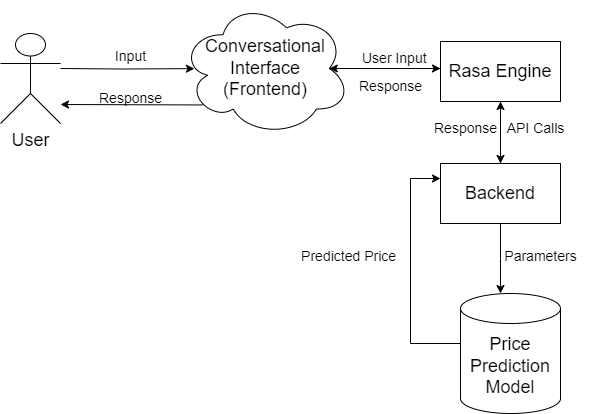
\includegraphics[width=0.8\textwidth]{Midsem.drawio.png}
    \caption{System Architecture of the Conversational Used Car Price Predictor}
    \label{fig:architecture}
\end{figure}

The system works as follows:
\begin{enumerate}
    \item The user interacts with the system via a conversational interface in the frontend, providing details such as the car’s make, model, year, mileage, and other relevant information.
    \item These inputs are processed by the \textbf{Rasa Engine}, which handles Natural Language Processing (NLP) and conversation management.
    \item The \textbf{Rasa Engine} extracts relevant parameters from the user's input and sends them to the backend via API calls.
    \item The backend forwards these parameters to the \textbf{Price Prediction Model}, which estimates the car's price based on the input features using a trained machine learning model.
    \item SHAP (SHapley Additive exPlanations) is applied to provide an explanation of how each input feature, such as mileage or car age, contributes to the predicted price.
    \item The backend returns both the predicted price and the explanation of the most significant contributing factor to the frontend.
    \item The predicted price and the SHAP-based explanation are then displayed to the user through the chat interface.
\end{enumerate}

This architecture ensures that the system is both interactive and explainable, allowing users to not only receive price predictions but also understand the reasoning behind them.

\section{Data Preprocessing}
\begin{justify}
Data preprocessing is a critical step to ensure that the machine learning model is provided with clean and well-structured data. Below are the detailed steps undertaken for preprocessing the dataset used in this project:

\subsection{Dataset Acquisition}
The dataset for this project was sourced from \textbf{Kaggle} in 2023, under the name \texttt{cardekho\_dataset}. It contains a wide variety of features related to used cars, including attributes such as the brand, model, year, mileage, and selling price, which are essential for predicting the value of used cars.

\subsection{Dropping Unnecessary Columns}
Certain columns in the dataset were deemed irrelevant or redundant for our analysis. For example:
\begin{itemize}
    \item The column \texttt{"Unnamed: 0"} was an irrelevant index and was removed.
    \item The \texttt{"car\_name"}  and \texttt{seller\_type} columns, though informative, were redundant and did not contribute significantly to the model's predictive power.
\end{itemize}

\subsection{Converting Vehicle Age to Year of Manufacture}
To standardize the data, the \texttt{vehicle\_age} column was converted to \texttt{year\_of\_manufacture}. This was done using the following formula:
\[
\texttt{year\_of\_manufacture} = 2023 - \texttt{vehicle\_age}
\]
After the conversion, the original \texttt{vehicle\_age} column was dropped from the dataset.

\subsection{Filtering Popular Car Models}
The dataset was filtered to retain only those car models that had more than 300 entries. This filtering ensures that the machine learning model is trained on a sufficiently large number of samples for each car model. The filtering process involved:
\begin{itemize}
    \item Calculating the frequency of each car model using \texttt{value\_counts()}.
    \item Retaining only models with more than 300 entries to ensure robust model training.
\end{itemize}

\subsection{Feature and Target Definition}
For the machine learning model:
\begin{itemize}
    \item \texttt{X} (features): Defined by dropping the columns \texttt{selling\_price}.
    \item \texttt{y} (target): Defined as the \texttt{selling\_price} of the car, which the model aims to predict.
\end{itemize}

\subsection{Handling Categorical Columns}
Several features in the dataset were categorical in nature, such as:
\begin{itemize}
    \item \texttt{fuel\_type}
    \item \texttt{transmission\_type}
    \item \texttt{brand}
    \item \texttt{model}
\end{itemize}
These categorical variables needed to be converted into numerical format using encoding techniques for compatibility with machine learning algorithms. The \texttt{OneHotEncoder} was applied to these features to convert them into binary (0/1) variables.

\subsection{Data Splitting}
The dataset was split into training and test sets in an 80:20 ratio using the \texttt{train\_test\_split()} function from \texttt{scikit-learn}. This ensures that the model is trained on 80\% of the data while the remaining 20\% is used to evaluate the model's performance. A \texttt{random\_state=42} was set to ensure reproducibility of results.

\subsection{Preprocessing Pipeline}
To streamline preprocessing, a pipeline was implemented using \texttt{ColumnTransformer} from \texttt{scikit-learn}. This pipeline applies \texttt{OneHotEncoder} to categorical columns while allowing other features to pass through unchanged:
\begin{quote}
\texttt{ColumnTransformer(transformers=[('cat', OneHotEncoder(handle\_unknown='ignore', sparse\_output=False), categorical\_cols)], remainder='passthrough')}
\end{quote}
This preprocessing pipeline ensures that the categorical variables are encoded appropriately, making the data suitable for training the machine learning model.

\end{justify}

\section{Model Training Process}
\begin{justify}
The model training process involves selecting an appropriate machine learning algorithm, setting up a pipeline for preprocessing and model training, tuning hyperparameters, and evaluating the model's performance through cross-validation. Below is a detailed explanation of each step involved in training the car price prediction model.

\subsection{Model Selection}
For this project, a \textbf{Random Forest Regressor} was chosen as the machine learning model for car price prediction. Random Forest is a powerful and flexible algorithm that handles both linear and non-linear relationships effectively. It is an ensemble learning method that constructs multiple decision trees during training and outputs the average prediction of the individual trees. This makes it robust and less prone to overfitting. Additionally, Random Forest works well with high-dimensional data and provides feature importance, making it suitable for our use case of price prediction.

\subsection{Pipeline Setup}
To ensure seamless and consistent data processing during both the training and testing phases, a \textbf{pipeline} was created using the \texttt{Pipeline} class from \texttt{scikit-learn}. The pipeline integrates the preprocessing steps (such as One-Hot Encoding for categorical features) and the Random Forest model into a single workflow. This approach guarantees that the same transformations applied to the training data are also applied to the test data, thereby avoiding data leakage.

\subsection{Hyperparameter Tuning}
To further optimize the performance of the Random Forest model, \textbf{RandomizedSearchCV} was employed for hyperparameter tuning. This method randomly samples a specified number of hyperparameter combinations from a predefined grid, allowing for efficient exploration of the hyperparameter space. The parameter grid for the Random Forest model included the following hyperparameters:
\begin{itemize}
    \item \texttt{n\_estimators}: Number of trees in the forest, tested with values of 100, 200, and 300.
    \item \texttt{max\_depth}: The maximum depth of each tree, with possible values of \texttt{None}, 10, 20, and 30.
    \item \texttt{min\_samples\_split}: Minimum number of samples required to split an internal node, tested with values of 2, 5, and 10.
    \item \texttt{min\_samples\_leaf}: Minimum number of samples required to be at a leaf node, with values of 1, 2, and 4.
\end{itemize}
The number of iterations for the random search was set to \texttt{n\_iter=10}, meaning 10 different combinations of hyperparameters were randomly selected and evaluated.

\subsection{Cross-Validation}
To ensure robust evaluation of the model's performance, \textbf{5-fold cross-validation} was used during hyperparameter tuning. In cross-validation, the data is split into 5 subsets (folds), and the model is trained on 4 of these folds while the remaining fold is used as the validation set. This process is repeated 5 times, with each fold serving as the validation set once. The model's performance is then averaged over the 5 iterations to give a more reliable estimate of how it will perform on unseen data.

\subsection{Model Training and Evaluation}
Once the optimal hyperparameters were selected using RandomizedSearchCV, the final model was trained on the full training dataset. The model was then evaluated on the test set using the \textbf{R² score}, which measures the proportion of variance in the target variable (car prices) that is explained by the model. The best Random Forest model achieved an \textbf{R² score of 0.925} on the test set, indicating strong predictive performance.

\subsection{Saving the Model}
To ensure that the trained model can be used for future predictions, it was saved using the \texttt{joblib} library. 

Saving the model allows for easy reuse without the need to retrain it every time a new prediction is required.

\end{justify}

\section{Identifying Influential Features}
\begin{justify}
One of the most valuable aspects of the machine learning model developed for predicting used car prices is its ability to provide explanations for its predictions. This is achieved using \textbf{SHAP} (SHapley Additive exPlanations), a method that assigns contribution values to each feature for a specific prediction. SHAP values allow us to break down and understand the role of each feature in driving the predicted price, offering insights into the decision-making process of the model.

\subsection{SHAP Value Calculation}
Once the model is trained, SHAP values are computed for each prediction. SHAP values quantify how much each feature contributes to pushing the predicted price higher or lower than the average model output. For example, if a feature such as mileage has a positive SHAP value, it indicates that it pushes the predicted price higher; conversely, a negative SHAP value suggests that the feature lowers the predicted price.

To compute SHAP values for this project, an \texttt{Explainer} object was created using the trained \texttt{RandomForestRegressor} model. The input data, after being transformed by the preprocessing pipeline, is passed to the explainer, which returns the SHAP values for each feature. These values represent how much each feature contributed to the predicted price for that particular car.

\subsection{Analyzing SHAP Values}
The SHAP values are organized into a \texttt{DataFrame} for easy interpretation. This provides a clear breakdown of each feature’s contribution to the predicted price. Features with positive SHAP values are identified as those that increase the predicted price, while those with negative SHAP values reduce the predicted price. The SHAP values are computed for each car, allowing for an in-depth analysis of individual predictions.

For instance, consider a test car such as the \textbf{BMW X5} (2020, Diesel, Automatic). The SHAP values provide insight into how much features like mileage, engine capacity, and fuel type contribute to the predicted price. This breakdown is valuable because it allows users to understand the key factors driving the price estimate for their car.

\subsection{Identifying the Most Influential Feature}
Once the SHAP values for a given prediction are calculated, the feature with the highest SHAP value is identified as the most influential factor in determining the predicted price for that specific car. This feature typically has the largest impact, either increasing or decreasing the predicted price. For example, if the \texttt{engine size} is identified as the most influential feature for a high-performance car like the \textbf{BMW X5}, it suggests that engine size is a key driver of the price for that vehicle.

\subsection{Percentage Contribution Calculation}
To provide a more intuitive understanding of the feature’s influence, the SHAP value of the most influential feature is divided by the predicted price to calculate its \textbf{percentage contribution}. This percentage represents how much the top feature contributes to the final predicted price. For instance, if the SHAP value for \texttt{engine size} is 30\% of the predicted price, it indicates that engine size is responsible for 30\% of the final car price prediction.
\newline

The system outputs both the predicted price and the feature with the highest contribution, along with the percentage of its influence. This breakdown gives users a clear explanation of why the predicted price is what it is, based on the car’s attributes. The transparency provided by SHAP values helps build trust in the model's predictions by offering explanations that are easy to understand.

\subsection{Example Results}
An example prediction for a car such as the \textbf{Hyundai i20} (2021, Petrol, Manual) would output the following results:
\begin{itemize}
    \item \textbf{Predicted Price}: Rs.656,002.24 (approximate).
    \item \textbf{Most Influential Feature}: remainder\_\_year\_of\_manufacture.
    \item \textbf{Percentage Contribution}: 24.36\%.
\end{itemize}
This means that 24.36\% of the predicted price can be attributed to the car's year of manufacture, highlighting the importance of this feature in the price determination process.

\section{Backend API Creation}
The backend of our application is built using Flask, a lightweight web framework for Python, which is designed to facilitate the creation of web applications. Flask allows us to develop RESTful APIs that serve predictions and insights derived from our machine learning model. The following outlines the structure and functionality of our API.

\subsection{Endpoints}
We have defined two primary endpoints for our application:

\begin{itemize}
    \item \textbf{/predict\_price}: This endpoint accepts various car attributes as query parameters and returns the predicted selling price of the car. Users can specify attributes such as brand, model, year of manufacture, kilometers driven, fuel type, transmission type, mileage, engine size, maximum power, and the number of seats.
    
    \item \textbf{/max\_contribution}: This endpoint also accepts the same car attributes as query parameters and returns the highest contributing feature to the predicted price along with its percentage contribution. This information helps users understand which specific attribute has the most significant impact on the price estimation.
\end{itemize}

\subsection{Input Handling}
Both endpoints utilize the GET method for input handling, allowing users to retrieve predictions based on the provided query parameters. The parameters are processed as follows:

\begin{itemize}
    \item The car attributes are retrieved from the query string of the request.
    \item The relevant data types are enforced; for example, integer and float values are cast appropriately to ensure the input data conforms to the expected formats.
\end{itemize}

\subsection{Response Format}
The API outputs predictions and contributions in JSON format. This format is widely used for data interchange and facilitates easy integration with frontend applications. JSON responses are structured to include relevant information for both predictions and contributions, allowing clients to effectively parse and utilize the data.

\subsection{Implementation Details}
The API is implemented in Python using the Flask framework. The core functionalities include loading a pre-trained machine learning model and using it to make predictions based on user input. Below is an overview of the main components:

\begin{verbatim}
from flask import Flask, request, jsonify
import pandas as pd
import joblib
import shap

app = Flask(__name__)

# Load the complete pipeline from Google Drive
model_path = 'best_car_price_model.pkl'
loaded_pipeline = joblib.load(model_path)
\end{verbatim}

The model is loaded using the Joblib library, which is efficient for handling large data. 

The function \texttt{predict\_price} is responsible for making predictions based on the input data. It transforms the input into a DataFrame format and passes it to the model for prediction. Similarly, the function \texttt{get\_max\_contribution} utilizes SHAP (SHapley Additive exPlanations) to analyze the model's predictions and determine the most influential feature contributing to the predicted price.

The API endpoints are defined as follows:

\begin{verbatim}
@app.route('/predict_price', methods=['GET'])
def price_prediction():
    ...
    
@app.route('/max_contribution', methods=['GET'])
def max_contribution():
    ...
\end{verbatim}

Each endpoint retrieves input parameters from the query string, processes them, and returns the corresponding predictions or contributions in JSON format.

Finally, the Flask application runs with debugging enabled, allowing for easier identification of issues during development:

\begin{verbatim}
if __name__ == '__main__':
    app.run(debug=True)
\end{verbatim}

This setup provides a robust and flexible backend API that can be easily extended or modified to accommodate additional features and functionalities in the future.


\end{justify}

\section{Chatbot Development using Rasa}
In this section, we describe the development of a rule-based chatbot using the Rasa framework. The chatbot is designed to assist users in predicting the price of a car based on its brand, model, and other attributes. The following subsections outline the key components and functionalities of the chatbot, including its configuration, intents, entities, responses, and custom actions.

\subsection{Framework Overview}
Rasa is an open-source framework for building conversational AI applications. It allows developers to create both rule-based and machine-learning-driven chatbots. In our case, we use Rasa's rule-based functionality to design a chatbot that can store and process car details, such as the brand and model, and provide predictions based on those details.

\subsection{Intents Overview}

In a natural language understanding (NLU) system, intents refer to the user’s goal or purpose behind a particular input. For the Car Price Prediction Chatbot, we designed a set of intents to handle different types of user queries. These intents enable the chatbot to understand and respond appropriately to user inputs. Below is a detailed explanation of each intent.

\textbf{Greet}: This intent is used when the user initiates a conversation or greets the chatbot. It helps the chatbot recognize when a user is saying “hello” or trying to begin an interaction.

\textbf{Examples}:
\begin{itemize}
    \item "Hey"
    \item "Hello"
    \item "Good morning"
    \item "Hi there"
\end{itemize}

\textbf{Goodbye}: This intent is activated when the user wishes to end the conversation. The chatbot recognizes farewell phrases and responds accordingly by concluding the interaction.

\textbf{Examples}:
\begin{itemize}
    \item "Goodbye"
    \item "See you later"
    \item "Bye"
    \item "Take care"
\end{itemize}

\textbf{Affirm}: This intent is triggered when the user confirms or agrees with something. It’s useful when the chatbot asks a question and expects a "yes" or an agreement from the user.

\textbf{Examples}:
\begin{itemize}
    \item "Yes"
    \item "Of course"
    \item "Indeed"
    \item "Sounds good"
\end{itemize}

\textbf{Deny}: This intent is used when the user disagrees or negates a statement or question. It helps the chatbot understand when the user is not in agreement.

\textbf{Examples}:
\begin{itemize}
    \item "No"
    \item "Not really"
    \item "I don't think so"
    \item "Incorrect"
\end{itemize}

\textbf{Bot Challenge}: This intent occurs when a user questions the chatbot’s identity, either asking whether it’s a bot or a human. The chatbot responds with information about its nature or confirms that it is indeed a bot.

\textbf{Examples}:
\begin{itemize}
    \item "Are you a bot?"
    \item "Am I talking to a bot?"
    \item "Are you human?"
\end{itemize}

\textbf{Inform}: This intent is used when the user provides details about their car. This can include the car’s brand, model, mileage, and other attributes. The chatbot uses this intent to collect the necessary details to predict the car price.

\textbf{Examples}:
\begin{itemize}
    \item "My car is a Hyundai Creta"
    \item "I have a Maruti Suzuki Swift"
    \item "The model is Ford Ecosport and the mileage is 18 km/l"
    \item "I drive a Tata Nexon"
\end{itemize}

\textbf{Stop}: This intent is used to end the conversation, often when the user says they are done interacting with the chatbot. The chatbot can gracefully close the conversation and stop any ongoing tasks.

\textbf{Examples}:
\begin{itemize}
    \item "Stop"
    \item "Exit"
    \item "Quit"
    \item "Cancel"
\end{itemize}

\textbf{Ask SHAP}: This intent is triggered when the user asks about the factors that contribute the most to a car’s price. SHAP (SHapley Additive exPlanations) is a method used in machine learning to explain the output of a model. This intent helps the chatbot explain what factors impact the car's price prediction.

\textbf{Examples}:
\begin{itemize}
    \item "What contributes the most to the price?"
    \item "Which feature affects the price the most?"
    \item "What features impact the price of a car?"
\end{itemize}

\textbf{Ask Mileage}: This intent is triggered when the user asks about car mileage. The chatbot responds with an explanation of what mileage means and how it affects the car's pricing.

\textbf{Examples}:
\begin{itemize}
    \item "What is mileage?"
    \item "Can you explain mileage?"
    \item "What does mileage mean in a car?"
\end{itemize}

\textbf{Ask Value Calculation}: This intent is used when a user inquires about how the value of a car is determined. The chatbot explains how factors like age, mileage, brand, model, etc., contribute to the overall price of the car.

\textbf{Examples}:
\begin{itemize}
    \item "How is the value of a car calculated?"
    \item "What factors determine a car's price?"
    \item "Can you explain how car pricing works?"
\end{itemize}

\textbf{Ask Engine Capacity}: This intent is triggered when the user asks about the engine capacity of a car. This intent helps the chatbot explain what engine capacity is and its role in pricing.

\textbf{Examples}:
\begin{itemize}
    \item "What is engine capacity?"
    \item "Tell me about the engine capacity."
    \item "What does engine capacity mean?"
\end{itemize}

\textbf{Ask Maximum Power}: This intent is activated when the user asks about the maximum power of the car's engine. This helps the chatbot explain the relevance of engine power in car pricing.

\textbf{Examples}:
\begin{itemize}
    \item "What is maximum power?"
    \item "Tell me about the maximum power of the car."
    \item "Can you explain maximum power?"
\end{itemize}




\begin{thebibliography}{9}

\bibitem{rasa}
Rasa Technologies, ``Rasa Documentation,'' \textit{Rasa}, 2023. [Online]. Available: \texttt{https://rasa.com/docs/}
\bibitem{flask}
Armin Ronacher, ``Flask Documentation,'' \textit{Flask}, 2023. [Online]. Available: \texttt{https://flask.palletsprojects.com/}


\bibitem{shap-doc}
SHAP Documentation, ``SHAP (SHapley Additive exPlanations),'' 2023. [Online]. Available: \texttt{https://shap.readthedocs.io/en/latest/}

\bibitem{randomforest}
Leo Breiman, ``Random Forests,'' \textit{Machine Learning}, vol. 45, no. 1, 2001, pp. 5-32. [Online]. Available: \texttt{https://link.springer.com/article/10.1023/A:1010933404324}

\bibitem{randomforest-doc}
Scikit-learn, ``Random Forests,'' 2023. [Online]. Available: \texttt{https://scikit-learn.org/stable/modules/ensemble.html-random-forests}

\end{thebibliography}

\end{document}
